\chapter{実験}
\label{chap:experiment}
第\ref{chap:proposal}章で述べた提案手法の有効性を検証するために,BAIR Push Dataset\cite{ebert2017selfsupervised}を用いて評価実験を行った.本章では実験の内容について説明した後に実験結果について述べる.

\section{実験内容}
第\ref{chap:proposal}章で述べた提案手法とベースラインの比較を行う.ベースラインは第\ref{chap:prerequisite}章で述べたシンプルなDSSMとし,状態ベクトルの次元を64, 256, 512, 1024の4通りに変えて実験を行う.提案手法は64次元と512次元の二階層の状態ベクトルを持つモデルと,64次元と512次元と1024次元の三階層の状態ベクトルを持つモデルとした.ベースラインと提案手法の実装の差は必要最小限にとどめ,どちらも学習時には10フレーム先までの予測を行った.またパラメータの最適化にはそれぞれ確率的勾配降下法アルゴリズム Adam\cite{kingma2014adam} を用いた.評価の際には,定量評価として予測誤差(負の対数尤度)を測り,合わせて定性評価も行う.

\subsection{ベースラインの実装}
深層学習フレームワークPytorch\cite{pytorch}と,深層生成モデルライブラリPixyz\cite{pixyz}を主に用いた.学習用データの読み込みとその最適化には深層学習フレームワークTensorFlow\cite{tensorflow}を用いた.また実装では,DSSMを用いた強化学習手法であるPlaNetの公開実装\cite{planet}を参考にした.
まずベースラインの実装を説明した後,提案手法の実装について述べる.

\subsubsection{モデルアーキテクチャ}
ベースラインは4つの部分モデルから構成される.
\begin{itemize}
    \item デコーダー $p(s_t|x_t)$
    \item エンコーダー $q(x_t|h_t)$
    \item 遷移モデル(事前分布) $p(s_t|s_t-1, a_t)$
    \item 遷移モデル(事後分布) $q(s_t|s_t-1, a_t, h_t)$
\end{itemize}

遷移モデル(事前分布)とデコーダーが生成モデルに相当し,提案手法のグラフィカルモデルの実践部分を表しす.遷移モデル(事後分布)とエンコーダーが推論モデルに相当し,提案手法のグラフィカルモデルの点線部分を表している.

\begin{figure}[tp]
    \centering
    \subfloat[デコーダーとエンコーダーのアーキテクチャ]{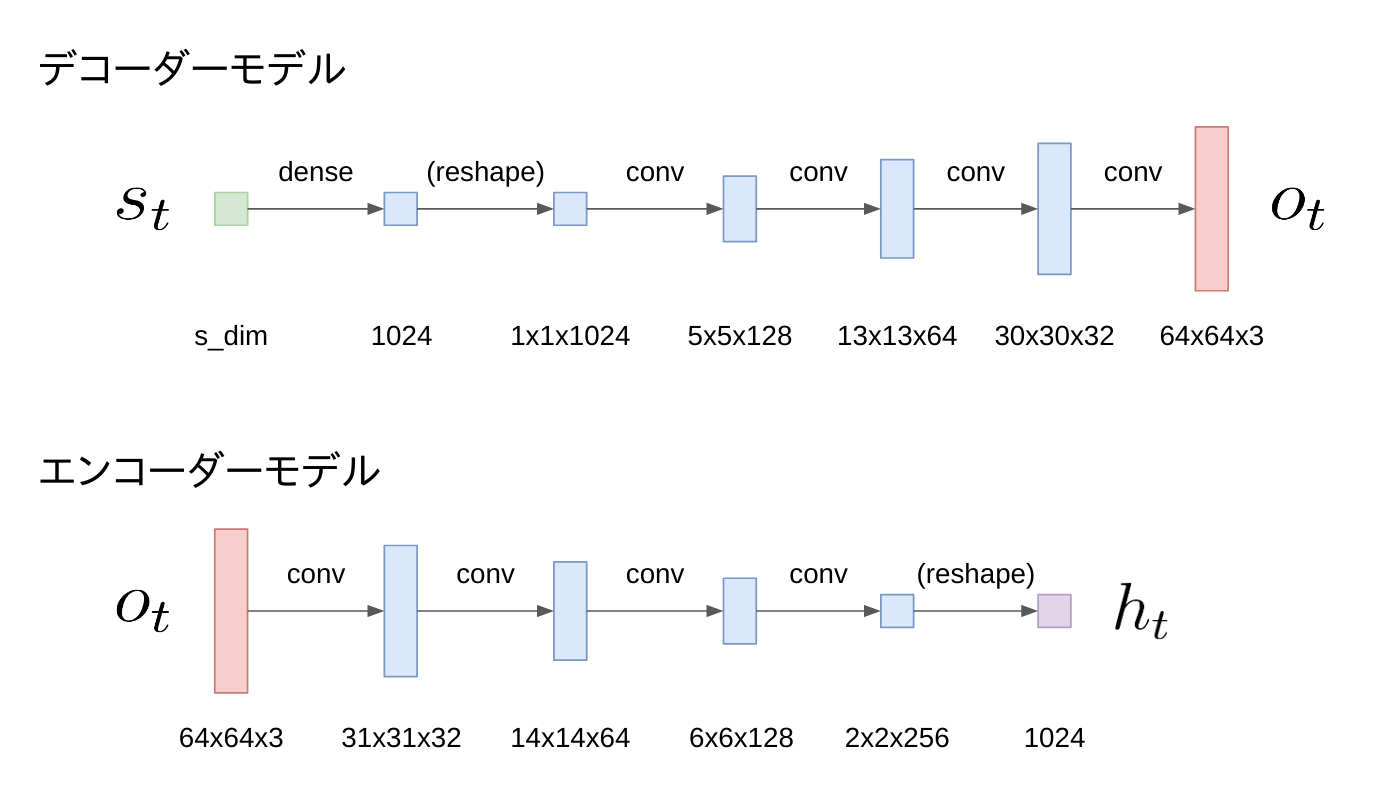
\includegraphics[clip, scale=0.25]{./figures/arch_encdec.png}
    \label{fig:arch_encdec}}
    \\
    \subfloat[遷移モデルのアーキテクチャ]{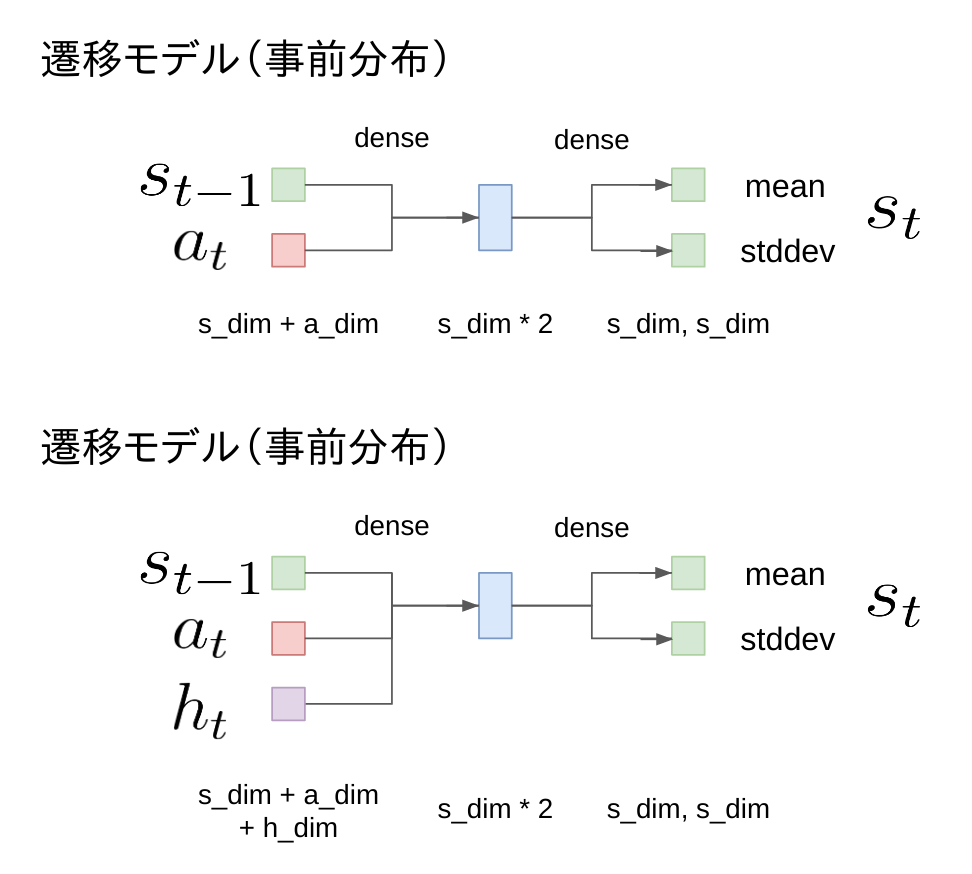
\includegraphics[clip, scale=0.25]{./figures/arch_trans.png}
    \label{fig:arch_trans}}
    \caption[モデルアーキテクチャ]{モデルアーキテクチャ.「dense」は全結合層,「conv」は畳み込み層,「reshape」は変数の変形を意味する.}
    \label{fig:arch}
\end{figure}
\begin{description}

    \item[デコーダー・エンコーダー]\mbox{}\\

図(\ref{fig:arch_encdec})にアーキテクチャの模式図を示す.PlaNetに倣い,デコーダー/エンコーダーモデルにはWorldModel\cite{ha1803world}の論文中に記載されているモデルを採用した.デコーダーは各時刻の状態ベクト$s_t$を全結合層で1024次元の隠れ変数に変換したあと,4層の逆畳み込み層で観測画像と同じサイズである64x64サイズのRGB画像に変換する.出力は各ピクセルごとに正規分布をおくが,本研究では簡単のためその分散はそれぞれ1に固定している.
エンコーダーは各時刻の観測を4層の畳み込み層と1層の全結合層で1024次元の隠れ変数$h_t$に変換する.

本研究では,状態変数の次元を変えた際にも隠れ層のパラメータ数などは一切変えなかった.

    \item[遷移モデル]\mbox{}\\
図(\ref{fig:arch_trans})にアーキテクチャの模式図を示す.遷移モデルには,ある時刻の状態ベクトル$s_t$を生成過程に従って生成する事前分布モデルと,ある時刻の観測$o_t$も与えられたときに$s_t$を推論する事後分布モデルの2種類を用意する.

この2つのモデルはアーキテクチャはほとんど共通で入力とするデータだけが違い,事前分布モデルでは一つ前の時刻の状態$s_{t-1}$と行動$a_t$を入力とするが事後分布ではそれに加えその時刻の観測$o_t$をエンコードして得たデータ$h_t$を入力とする.出力はどちらのモデルも次の時刻の状態ベクトルの分布の母数(平均と標準偏差)である.
アーキテクチャは,入力情報をすべて連結して一度全結合層で変換したものを平均を求める全結合層と標準偏差を求める全結合層のそれぞれで変換し,求めたい分布の平均と標準偏差を出力する.

\end{description}

\subsubsection{学習の安定化}
潜在変数の次元を大きくした際,学習の初期段階でカルバックライブラー距離の計算値が発散することがよく起こる.これは遷移モデルが次の時刻の状態ベクトルの分布の標準偏差として0に非常に近い値を出力してしまった結果(丸め誤差が発生して)カルバックライブラー距離の計算時にゼロ除算が発生してしまうためである.この問題は遷移モデルが出力する標準偏差に下限を設けることで解決することができる.今回の実験では潜在変数の次元を1024次元にした際にこのカルバックライブラー距離が学習開始後直ちに発散する問題が発生したので,標準偏差の下限値を$10^{-7}$とすることで学習をある程度継続することができた.ただし標準偏差に下限を設けることは経験的に学習を難しくすることが予備実験でわかっていたので,他の条件での実験の際には適用しなかった.

\subsection{提案手法の実装}
提案手法はベースラインの節で説明した部分モデルをほぼそのまま用いる.二階層目以上の第i層では,各遷移モデルの入力として一時刻前の状態変数$s^i_{t-1}$と行動$a_t$だけでなく,一つ低次元の層の同じ時刻の状態ベクトル$s^{i-1}_t$も入力とする.また,提案手法では,パラメータを固定している層の状態ベクトルのサンプリングには,モデルの評価時の設定に合わせて常に事前分布を用いている.これは,パラメータを固定している層はそれ以上学習されないために,事前分布より良い表現が下の階層に渡されることはなく,むしろ事前分布で足りない表現を積極的に下の階層の学習で獲得できるようにするためである.
その他はベースラインの実装と変えていない.


\section{実験結果}

簡単のため,ここから状態変数の次元を64にしたベースラインモデルを「ベースライン(64)」,状態変数の次元を64と512にした提案手法モデルを「提案手法(64 + 512)」などと呼ぶ.

\subsection{定量評価(尤度)}

\begin{figure}[tp]
    \begin{center}
        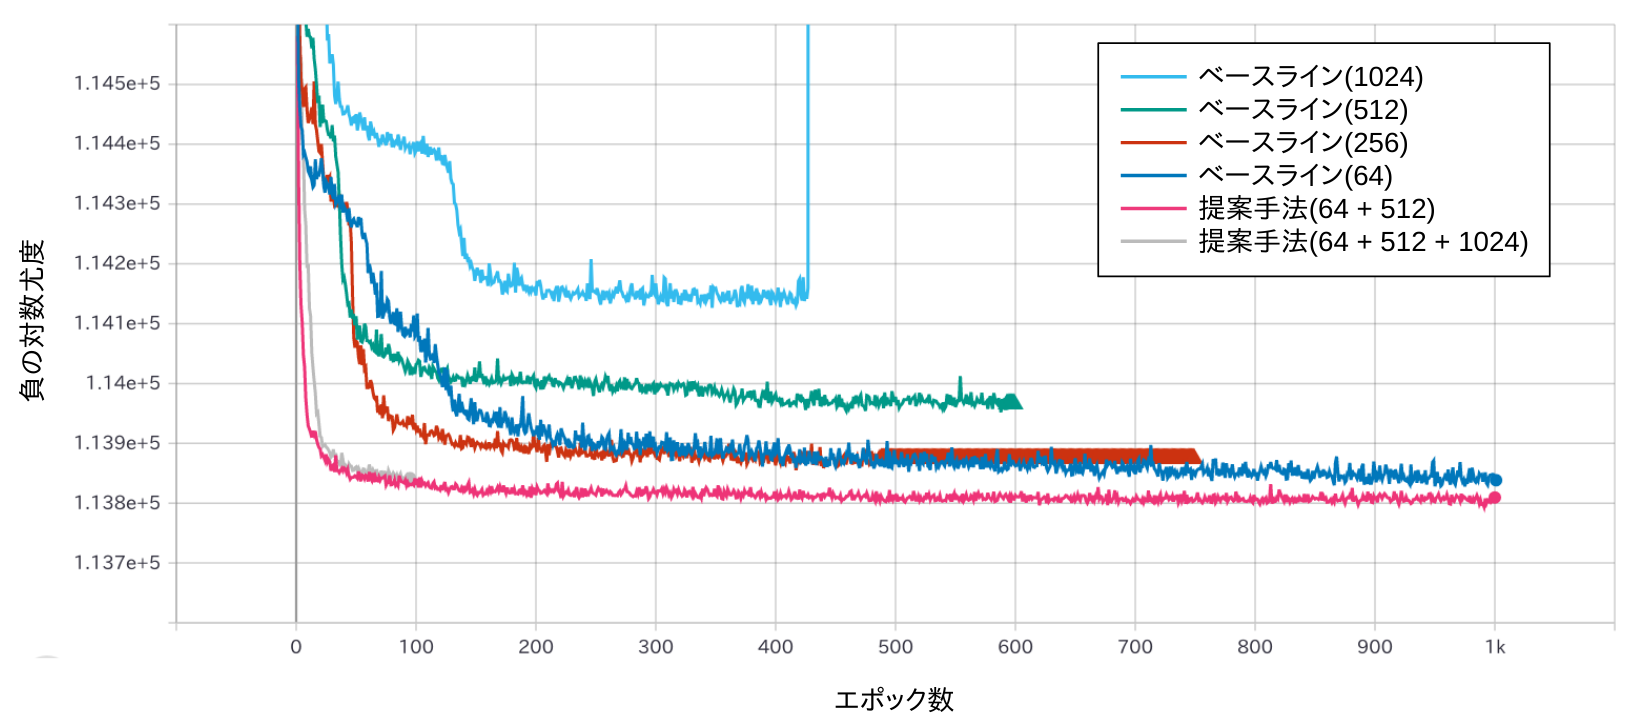
\includegraphics[width=\linewidth]{./figures/curve.png}
        \caption[提案手法の学習曲線]{ベースラインと提案手法の学習曲線}
        \label{fig:curve}
    \end{center}
    \end{figure}

\begin{table}[tbp]
    \begin{center}
    \caption{手法ごとの定量評価指標(尤度)}
    \begin{tabular}{|c||c|} \hline
      手法 & 負の対数尤度 \\ \hline \hline
      ベースライン(64) & $1.1384 \times 10^5 $ \\ \hline
      ベースライン(256) & $1.1387 \times 10^5 $ \\ \hline
      ベースライン(512) & $1.1397 \times 10^5 $ \\ \hline
      ベースライン(1024) & $1.1416 \times 10^5 $ \\ \hline
      提案手法(64 + 512) & $\bm{1.1381 \times 10^5 }$ \\ \hline
      提案手法(64 + 512 + 1024) & $1.1383 \times 10^5$ \\ \hline
    \end{tabular}
    \label{table:evaluation}
    \end{center}
  \end{table}
  

図(\ref{fig:curve})は,ベースラインと提案手法の学習時の評価用データでの負の対数尤度の値の推移をプロットしたもの(学習曲線)である.ただし提案手法(64 + 512)は一階層部分に1000 epoch 学習したベースライン(64)を用いており,学習曲線としてプロットされているのは二階層部分の学習時の負の対数尤度である.同様に提案手法(64 + 512 + 1024)は一階層部分に1000 epoch 学習したベースライン(64)を,二階層部分に1000 epoch 学習した提案手法(64 + 512)を用いており,学習曲線としてプロットされているのは三階層部分の学習時の負の対数尤度である.また表(\ref{table:evaluation})に最終的な負の対数尤度を示す.

まず図(\ref{fig:curve})について,ベースライン(512)と提案手法(64 + 512)との比較から,二階層にすることで潜在変数の次元を512次元と大きくした際にもうまく学習が進むようになったことがわかる.これは,高次元の状態変数の学習時に学習済みの低次元の状態変数の情報を用いることで狙い通り学習が安定したためだと考えられる.次にベースライン(64)と提案手法(64 + 512)の比較から,高次元の潜在変数で学習させたことによってより高い尤度の映像を生成できるようになったことがわかる.これは潜在変数を高次元にした方が多くの情報を保持しやすく,適切に学習が進みさえすれば予測性能が向上しやすくなるためだと考えられる.最後に三階層の提案手法(64 + 512 + 1024)について見ると,ベースライン(1024)と比較し明らかに学習が進んだものの,ベースライン(64 + 512)と比較して精度の改善は見られず,潜在変数の次元を大きくすることだけでは精度の向上には限界があるということが伺える.

\subsection{定性評価}
図(\ref{fig:compare_ab}),図(\ref{fig:compare_cd})は評価用データで10フレームの行動条件付き映像予測により生成された映像のサンプルで,正解映像とベースライン(64)による予測映像,提案手法(64 + 512)による予測映像を比較している.どちらのモデルもロボットアームの位置はほぼ正しく予測ができているが,環境中の物体の見た目には差が見られた.図(\ref{fig:pred_a}), 図(\ref{fig:pred_b})を見ると,ベースラインでは環境中の物体の輪郭がぼやけて灰色がかっているのに対し,提案手法では特に物体が密集していない場合に比較的物体一つ一つの生成が鮮明になっていることが見て取れる.これは潜在変数の次元を大きくし保持できる情報を増やすことに成功したためだと言える.しかしフレームごとの見た目には改善が見られたものの,物理的な操作についての予測はあまり改善が見られなかった.図(\ref{fig:pred_c})では,正解映像ではロボットアームの移動によって中央の緑の物体の姿勢を変えているが,そもそもベースラインではその物体を生成できておらず,提案手法でも僅かに黒っぽい点として表されている程度で姿勢の変化を読み取ることはできない.図(\ref{fig:pred_d})は,正解映像では滑らせるようにして2つの物体を近づけており,提案手法のでは2つの物体の輪郭が見られるが,机の色やロボットアームの色と途中から同化してその動きを追うことは困難である.このように物理的な操作の予測を改善するにはまず一フレーム一フレームの質を上げる必要があると考えられ,今回は物理的な操作の予測の改善はあまり見られなかった.最後に図(\ref{fig:pred_long})は,各モデルで学習時よりも長い30フレームの映像予測をした際の生成映像である.ベースライン・提案手法ともにロボットアームの動きはほぼ正解映像と一致しているが,ベースラインでは右端に映る物体が映像を予測するにつれて青色から緑色に変わってしまっているのに対し,提案手法は背景や周りの物体について一貫性が保たれていた.これは,潜在変数の次元が小さいまま性能をあげようとすると潜在表現に含まれる情報が密になりすぎて遷移時に遷移とは関係のない情報も変化させてしまいやすいという問題がある可能性があり,一方提案手法は高次元の潜在変数を使うためにそのような問題は生じなかったと考えられる.

% また図(\ref{fig:pred_a})では,水色の物体の予測位置が提案手法が生成した映像と正解映像とで少しずつずれているが,このことから画像を一画素ずつ潜在表現で記憶しているのではなく,物体の見た目と位置を別々に保存するように学習がすすんでいたことが伺える.

% 高次元で学習できるようになった.これは深層状態空間モデルの大きな問題点を克服できたと言える.

\begin{figure}[tp]
    \centering
    \subfloat[]{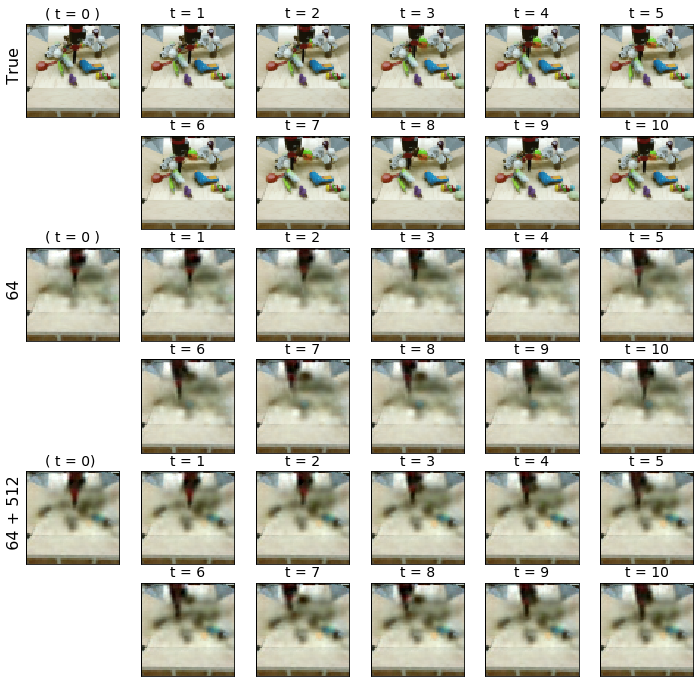
\includegraphics[clip, width=0.63\linewidth]{./figures/pred_a.png}
    \label{fig:pred_a}}
    \\
    \subfloat[]{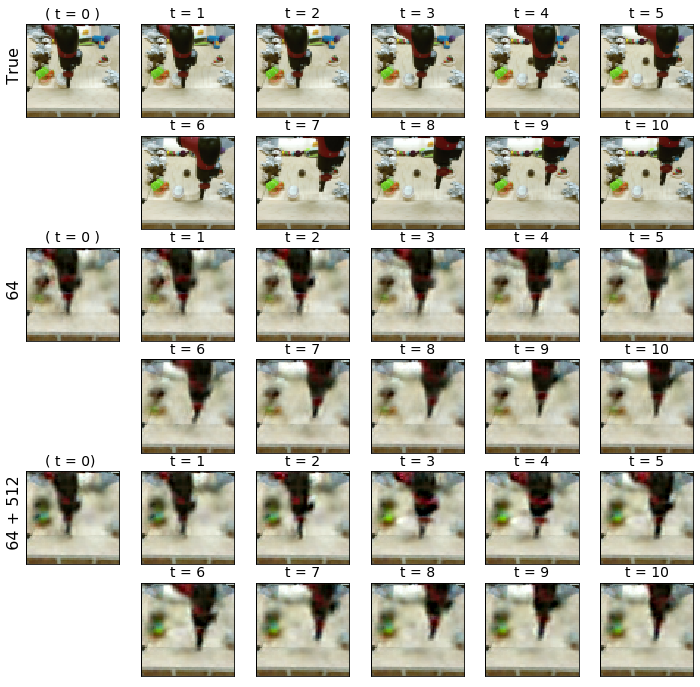
\includegraphics[clip, width=0.63\linewidth]{./figures/pred_b.png}
    \label{fig:pred_b}}
    \caption[映像予測結果1]{映像予測結果1.「True」が正解映像,「64」がベースライン(64)での予測結果,「64 + 512」が提案手法(64 + 512)での予測結果を示す.また$t = 0$は初期状態の推論時に与えられるフレームを示す.}
    \label{fig:compare_ab}
\end{figure}

\begin{figure}[tp]
    \centering
    \subfloat[]{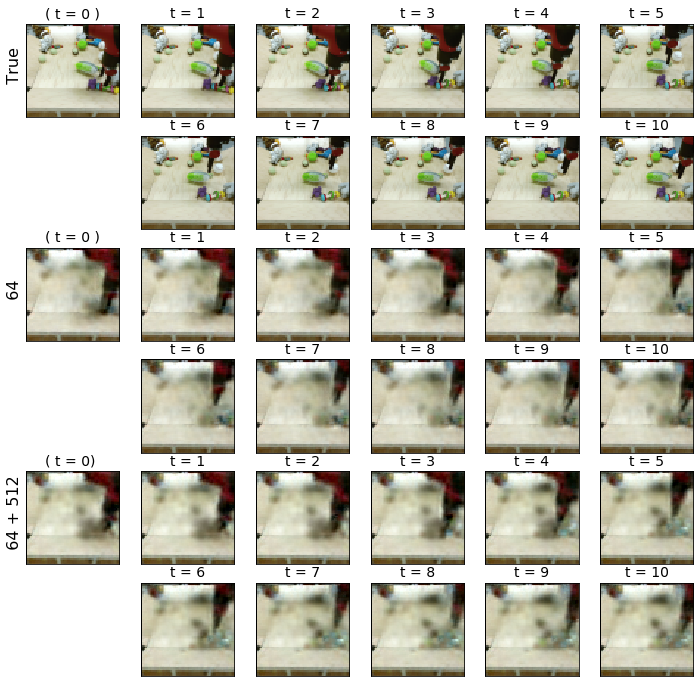
\includegraphics[clip, width=0.63\linewidth]{./figures/pred_c.png}
    \label{fig:pred_c}}
    \\
    \subfloat[]{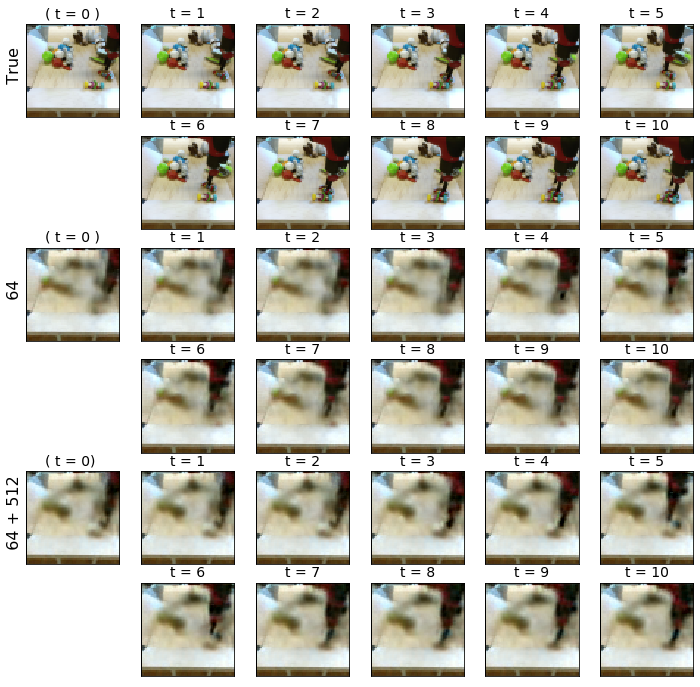
\includegraphics[clip, width=0.63\linewidth]{./figures/pred_d.png}
    \label{fig:pred_d}}
    \caption[映像予測結果2]{映像予測結果2.「True」が正解映像,「64」がベースライン(64)での予測結果,「64 + 512」が提案手法(64 + 512)での予測結果を示す.また$t = 0$は初期状態の推論時に与えられるフレームを示す.}
    \label{fig:compare_cd}
\end{figure}

\begin{figure}[tbp]
    \begin{center}
        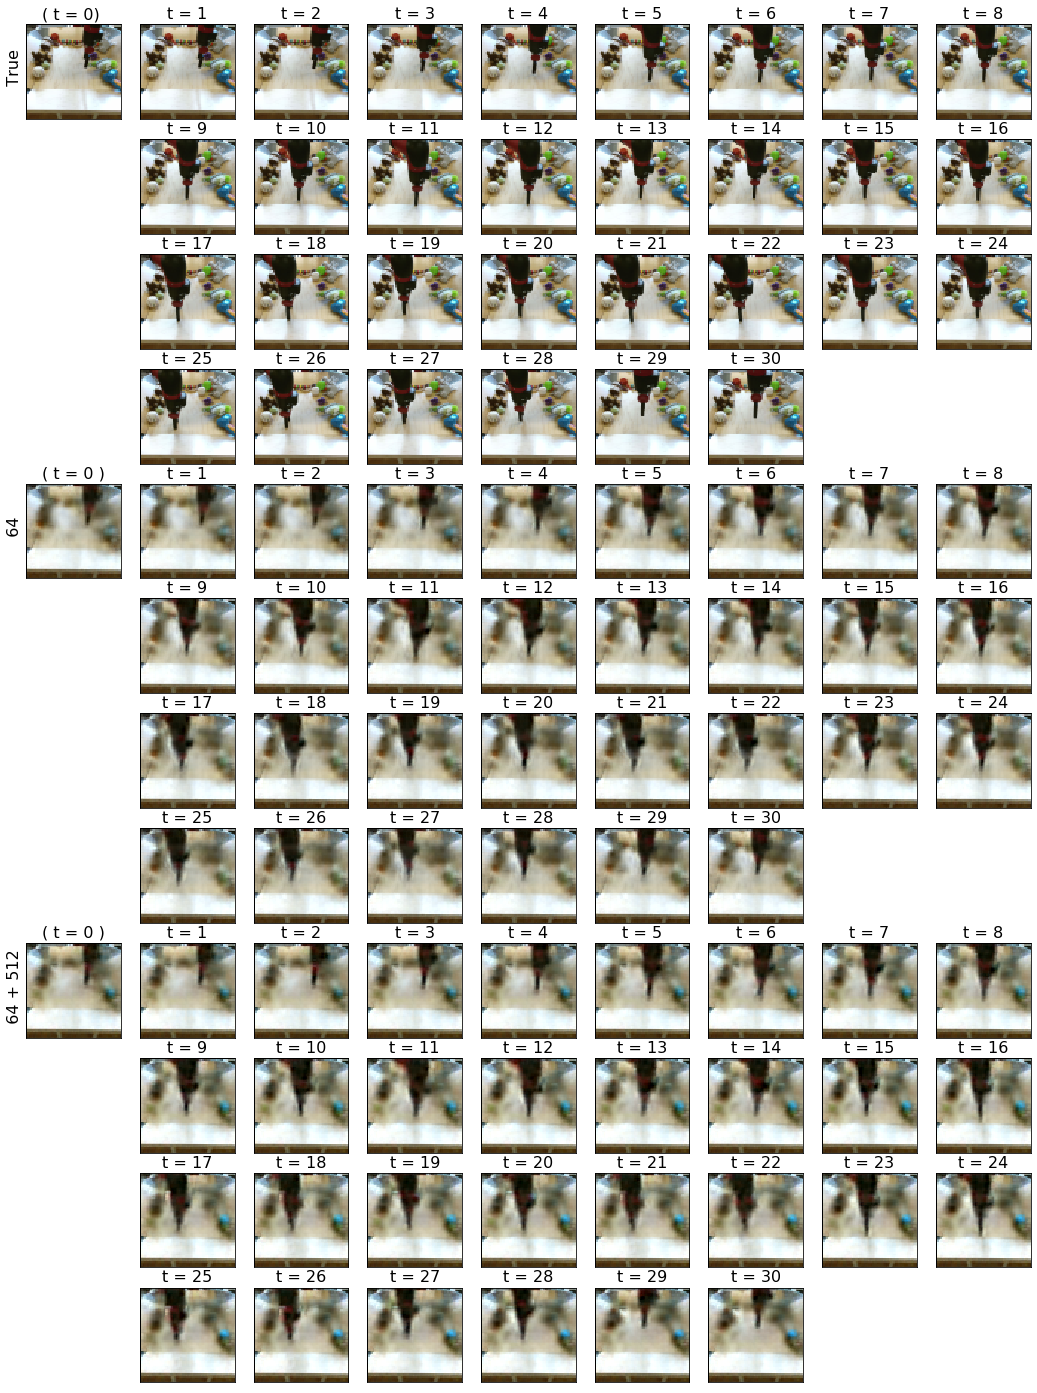
\includegraphics[width=0.95\linewidth]{./figures/pred_long.png}
        \caption[30フレームの予測結果の比較]{30フレームの予測結果の比較.「True」が正解映像,「64」がベースライン(64)での予測結果,「64 + 512」が提案手法(64 + 512)での予測結果を示す.また$t = 0$は初期状態の推論時に与えられるフレームを示す.}
        \label{fig:pred_long}
    \end{center}
\end{figure}

% 次元の大きさ ~ 情報量の大きさ 

% 高次元の潜在変数を用いたい場合は今回の手法は有効である.

% 三階層にしても学習は進むが,階層にして潜在変数の次元を大きくするだけでは性能の向上に限界がある.